\section{Introduction}
  Inverse pyramid:
  \begin{itemize}
    \item P1: Background
    \begin{enumerate}
      \item Inverse pyramid
      \item Last sentence: introduce the area of the title of your paper as a significant topic
      \item 5 refs (books, review papers, journals, no conf)
    \end{enumerate}
    \item P2-3: Background
    \begin{enumerate}
      \item Original classification: Support the objectives with each sentence
      \item Appreciate their work, their focus however different
      \item no technical words
      \item 10 refs (journal, conference papers)
    \end{enumerate}
    \item P4: Objectives
    \begin{enumerate}
      \item 1-3 objectives
      \item the first sentence: this paper presents
    \end{enumerate}
    \item P5: Outline
    % \item Start from importance of localization
    % \item importance of indoor localization
    % \item GPS-denied, that's why radio waves
    % \item Radio channels are time-varying, noisy and prone to different sources of failure
    % \item many solution has been proposed but my contributions are more significant
    % \item outline
  \end{itemize}
  % The radio waves ..
  % Since the use of \gls{rf} has become ubiquitous, it started being utilized in different applications varying from customer tracking indoors to robot localization. % more varying examples would be good.
  % Since its invention radio waves are
  % However it is available, the information can be extracted from is prone to (suffers from) being sparse and severely effected by infrasracture of environments where WiFi based systems are deployed.
  % Amongst all the applications that WiFi signal can be used, robot localization is a problem where it is required to have higher level of success in localization accuracy and shorter localization time.
  % \textit{The main contributions of this paper is that the proposed technique can handle sparse, noisy RSS measurements acquired from the off-the-shelf AP's under LoS and NLoS situations, while achieving comparable localization accuracy to thes state-of-the-art methods.}
  %
  % The success of the systems relying on the WiFi signal, in general, suffers from the phenomenon called Multipath Effect in which the AP is not in the direct line of sight and the EM waves from the AP where the received signal is propagated through non-line-of-sight, i.e.~concrete and glass walls.
  % Although there is some effort to either model or estimate the Multipath Effect to componsate its effects on the systems~\cite{cai2015identification}, it is still an open problem in the field in order to achieve the same level of success under NLoS observations.
  % %One way to componsate the multipath effect is to find out the first the time epoch the signal is acquired; however, some of these operations require significant change in hardware so that  \# \#.
  % \textit{The proposed system can inherently handle multipath effect, since machine not only can reduce complexity of overall design of the system but also can capture deeper information from the radio maps.}
  % % \textit{More explanation regarding the multipath effect is needed here to emphasize that machine learning algorithms can inherently handle it.}
  %
  % Another problem with the WiFi signal which makes it difficult to employ it as the main information source is that the signal acquired is not reliable.
  % Figure~\ref{fig-variance} shows the acquired RSS information acquired with stationary client from the AP's both line-of-sight and non-line-of-sight positions in time.
  % The figure clearly depicts that even for stationary clients, the RSSI readings greatly deviates from the mean in time.
  % % \#\textit{gotta mention that deviation makes it not reliable}.
  % To be able to extract relatively reliable information, some hardware and software changes proposed to incorporate Channel State Information (CSI) provided by Orthogonal Frequency-Division Multiplexing (OFDM) forming WiFi protocol.
  % As~\cite{gao2015channel} suggests/proves, the CSI information provides significantly reliable information.
  % However, to be able to acquire CSI information, a specific type of NIC should be used with a specific type of firmware.
  % This makes it hard to deploy proposed system on Embedded-devices, IoT's and robotic systems.\textit{, while the proposed system can be deployed to almost-any arbitrary system thanks to the simplicity of the design.}
  %
  % % \textit{Nail the idea Machine Learning stuff can be deployed practically everywhere}
  %
  % The paper is organized as follows.
  % The following section reviews the literature regarding robot localization with WiFi signal.
  % In Sec.~\ref{sec-PF}, we formalize the problem.
  % Section~\ref{sec-SD} thoroughly explains the proposed system.
  % The experimentation and the results are  in Sec.~\ref{sec-EX}.
  % We outline our observation and conclusions in the final section.
  % This section will cover the existing fingerprinting-based indoor radiolocation systems.
  % Fingerprinting-based radiolocation systems had been surveyed many times~\cite{he2016wi, honkavirta2009comparative} with different scopes due to its popularity in both academia and the industry.
  %
  % RADAR~\cite{radar}: One of the earliest
  %
  % EZ~\cite{chintalapudi2010indoor} employs the log-distance model with a Genetic Algorithm based optimizer along with a \gls{pf} fusing location estimates with inertial measurements.
  %
  % Horus~\cite{youssef2005horus} is one of the early methods relying on Bayes' theorem and spatial clustering.
  % While Horus achieves a significant improvement in localization accuracy, the computational complexity
  %
  % Zee~\cite{rai2012zee}: off-the-shelf hw, crowdsourcing
  % Many of the previous systems employ spatial pattern of the fingerprints, while others use temporal pattern displayed by anchor nodes.
  %
  % %
  % % UnLoc~\cite{wang2012no}: zero supervising, no training; heavily depends on landmark extraction and dead reckoning. (mobile device)
  % % One of the recent advances is that to incorporate the hard-constraints induced by the environment infrasracture.
  % UnLoc~\cite{wang2012no} is an examplary instance falling into the former category.
  % The system aims for incorporating hard-constraints of the environment, namely, elevators, stairs, entrances, and the change in the fingerprint patterns; for instance, a significant drop of signal level of a specific anchor node in a specific region.
  %
  % Particle filter~\cite{biswas2010wifi}: PF, dead reckoning
  %
  % Zee~\cite{rai2012zee}: off-the-shelf hw, crowdsourcing
  %
  % While Bayesian framework was used to present the belief of the robot pose and construct signal map in the previous works, LiFS~\cite{yang2012locating} approximated the environment by a grid-based method.
  % The grids are then transformed to \textit{stress-free floor plan} where the grids were clustered based on walking-distance among each other rather than physical distance; due to the fact that in indoor settings not every neighboring grids are accessible from one to another within one step.
  % The fingerprints are then collected during a walk in the localization environment, as the proposed data acquisition algorithm labels fingerprints with the number of steps taken.
  % The signal map were then constructed with the observed fingerprints with a Multidimensional scaling technique~\cite{borg2005modern}.
  % % The fingerprints are then clustered with the same multiscaling algorithm, after a tedious preprosessing step.
  % After acquiring fingerprint space and stress-free floor plan, the correspondence between two information was then calculated to map one to another; thus, spatial information was tied to fingerprints of the AP's.
  % This work achieved comparable localization results but depending on
  %
  % ArrayTrack~\cite{xiong2013arraytrack}: One of the best
  %
  %
  % Walkie-Markie~\cite{shen2013walkie}: spatial-pattern
  %
  %
  % SpotFi~\cite{kotaru2015spotfi}: One of the best
  %
  %
  % %
  % % FP~\cite{he2016wi}: FP Survey
  % %
  % % Calibration-free~\cite{hossain2015survey}: Calibration-free survey
  % %
  % % General wireless~\cite{liu2007survey}: High number of citations
  %
  % % \subsection{Indoor Localization with Machine Learning}
  % kNN:~\cite{liu2007survey}
  %
  %
  %
  % Neural networks:~\cite{dayekh2010cooperative}
  %
  %
  % SVM:~\cite{wu2007location}
  %
  %
  % Deep-Fi~\cite{wang2016csi}: \gls{rbm}
  %
  % % \begin{itemize}
  % %   \item{RSS Based}
  % %   \item{CSI Based}
  % %   \item{TDOA Based}
  % %   \item{RTT Based}
  % % \end{itemize}
  %
  % In the scope of WiFi localization systems, it is still an open problem in the field of robotics to deal with this problem with off-the-shelf AP's, while resulting relatively higher localization results than other applications where NLoS observation can happen anytime.
  % \begin{figure}[thpb]
  %    \centering
  %    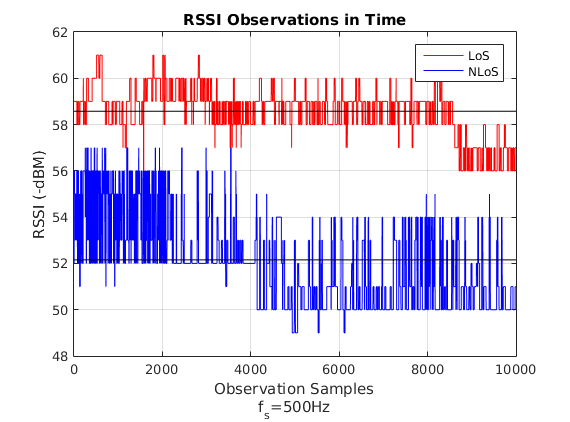
\includegraphics[width=\linewidth]{figures/rssi_variance.png}
  %    \caption{\label{fig:variance}RSSI readings of NLoS and LoS APs acquired with a stationary agent}
  % \end{figure}
